\documentclass{article}
\usepackage[utf8]{inputenc}
\usepackage[spanish]{babel}
\usepackage{hyperref}
\usepackage{url}

\title{Proyecto de investigación - Interrupciones}
\author{David Esteban Monsalve Pulgarin}
\date{\today}

\usepackage{natbib}
\usepackage{graphicx}
\graphicspath{ {images/} }

\begin{document}

\maketitle

\section{¿Qué es una interrupción en el contexto de los microprocesadores?}

\par
Las interrupciones son un mecanismo por el que un dispositivo externo puede provocar que el procesador interrumpa momentáneamente la ejecución del programa para atender su petición y luego continuar con el programa desde el punto en que lo había dejado. Estas se pueden ver como protocolos de comunicación a través de los cuales se pueden comunicar tanto los dispositivos de entrada y salida tales como los dispositivos de almacenamiento, mouse, teclado, entre otros con la unidad de procesamiento, a su vez estas actúan como mecanismos que por medio de esta comunicación con el procesador, se permite una interrupción temporal por parte del procesador y se transfiere el control a una interrupción que está solicitando este permiso y una vez ésta termine se vuelve a ejecutar el proceso originalmente anterior.En otras palabras una interrupción es una suspensión temporal de la ejecución de un proceso, para pasar a ejecutar una subrutina de servicio de interrupción, la cual, por lo general, no forma parte del programa, sino que pertenece al sistema operativo o al BIOS). Una vez finalizada dicha subrutina, se reanuda la ejecución del programa. 


\section{¿Se puede hablar de la historia de las interrupciones?}
\par
\vspace{5mm}
Las interrupciones surgen de la necesidad que tienen los dispositivos periféricos de enviar información al procesador principal de un sistema informático.La primera técnica que se empleó para esto fue el polling, que consistía en que el propio procesador se encargara de sondear los dispositivos periféricos cada cierto tiempo para averiguar si tenía pendiente alguna comunicación para él. Este método presentaba el inconveniente de ser muy ineficiente, ya que el procesador consumía constantemente tiempo y recursos en realizar estas instrucciones de sondeo.

\vspace{5mm}
\par
El mecanismo de interrupciones fue la solución que permitió al procesador desentenderse de esta problemática, y delegar en el dispositivo periférico la responsabilidad de comunicarse con él cuando lo necesitara. El procesador, en este caso, no sondea a ningún dispositivo, sino que queda a la espera de que estos le avisen (le “interrumpan”) cuando tengan algo que comunicarle (ya sea un evento, una transferencia de información, una condición de error, etc.).


\section{¿Que tipo de interrupciones existen?}
\subsection{Tipos de interrupciones}
\vspace{4mm}
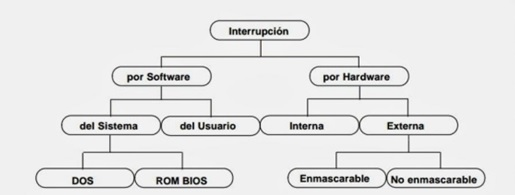
\includegraphics{interrupciones.jpg}
\vspace{5mm}

\section{¿Cómo se hace la implementación de interrupciones a nivel de hardware?}

\par
Estas interrupciones ocurren cuando un dispositivo necesita atencion del procesador y genera una señal electrica en la linea IRQ que tiene asignada. No son producidas por ninguna instrucción de un programa sino por las señales que emiten los dispositivos periféricos para indicarle al procesador que necesitan ser atendidos. Cuando el microprocesador accede a un periférico (disco duro, puerto de comunicación…), puede transcurrir algún tiempo antes de que los datos sean obtenidos o transmitidos. 

En los sistemas modernos se prefiere un funcionamiento mediante interrupciones, ya que éstas permiten mejorar la productividad del procesador, de forma que este último puede ordenar una operación de E/S y, en lugar de tener que realizar una espera activa, se puede dedicar a atender a otro proceso o aplicación hasta que el dispositivo esté de nuevo disponible, siendo dicho dispositivo el encargado de notificar al procesador mediante la línea de interrupción que ya está preparado para continuar/terminar la operación de E/S.

Existen dos clases de interrupciones por hardware:
\par


{\em \large Interrupcion enmascarable:} Significa que, bajo control del software, el procesador puede aceptar o ignorar (enmascarar) la señal de interrupcion.

{\em \large Interrupcion no enmascarable:} Significa que la interrupcion no puede ser deshabilitada por software. Este tipo de interrupciones ocurren cuando se recibe una señal en la pantalla NMI (Interrupcion no enmascarable) del procesador

\section{¿Cómo se implementan las interrupciones por software?}
\par
Este tipo de interrupciones son utilizadas tanto por el sistema operativo como por los progrmas de usuario que pueden instalar las suyas de manera particular. Las interrupciones por software son aquellas generadas por un programa en ejecución. Para generarlas, existen distintas instrucciones en el código máquina que permiten al programador producir una interrupción, las cuales suelen tener nemotécnicos tales como INT (por ejemplo, en DOS se realiza la instrucción INT 0x21 y en Unix se utiliza INT 0x80 para hacer llamadas de sistema).La interrupción por software, también denominadas llamadas al sistema, son aquellas generadas por un programa mientras este está ejecutándose. 

\par
El bus de control de la placa base dispone de líneas específicas para el sistema de interrupciones. Un PC típico dispone en su placa base de un controlador de interrupciones 8259 de Intel o de un circuito integrado análogo. Este dispositivo electrónico dispone de hasta 16 líneas IRQ, numeradas desde el 00 hasta el 15. En las nuevas placas base este circuito está integrado junto con el resto del chipset y permite hasta 24 interrupciones. Los procesadores de intel de la gama x86 y compatibles, disponen de una instruccion INT que permite generar por software cualquiera de los 256 tipos de interrupcion. En el IBM PC y XT existían 8 líneas de petición de interrupción manejadas por el controlador de interrupciones Intel 8259. Esta claro que dependiendo del sistema operativo se presentara un rendimiento diferente y se tienen distintas funcionalidades, y respecto al hardware en algunos dispositivos se cuentan con un mayor rango de asistencia para ejecutar las interrupciones. 

\section{Mostrar un ejemplo de interrupción usando la plataforma Arduino.}

\url{https://www.tinkercad.com/things/0r3fylaf4lQ}
\vspace{10mm}
\section{Cibergrafias}
\url{https://lcsistemasoperativos.wordpress.com/tag/interrupciones/}
\par
\vspace{2mm}
\url{https://es.wikipedia.org/wiki/InterrupciC3B3n}
\par
\vspace{2mm}
\url{https://www.cs.cinvestav.mx/TesisGraduados/2008/tesisLuisLeyva.pdf}
\vspace{2mm}
\par
\url{https://issuu.com/kevinaguilar13/docs/interrupciones.docx}

\end{document}
